\documentclass[10pt, a4papert, hidelinks]{article}

\usepackage{fancyhdr}

\usepackage{layout}
\textwidth = 400pt

%\setlength{\parskip}{1.6em}
%\setlength{\parindent}{1.25cm}

\usepackage[utf8]{inputenc}
\usepackage[english]{babel}
\usepackage{csquotes}
\usepackage{tabto}
\usepackage{textcomp}

\usepackage[left=3cm, right=3cm, top=3cm, bottom=4cm]{geometry}

\linespread{0.8}

\usepackage[
backend=biber,
style=numeric,
sorting=anyt
]{biblatex}
\addbibresource{./sources.bib}

\usepackage{setspace}
\onehalfspacing
% \doublespacing
\usepackage{booktabs}

\usepackage{amsmath}
\usepackage[dvipsnames]{xcolor}
\usepackage{mathtools}
\usepackage{amsfonts}
\usepackage{titlesec}
% \usepackage{pgfplots}
% \usepackage{pgfplotstable}
% \usepgfplotslibrary{statistics}
% \usepackage[
%   separate-uncertainty = true,
%   multi-part-units = repeat
% ]{siunitx}
% \usepackage{csvsimple}

\colorlet{lightgreen}{green!30}
\colorlet{rose}{red!30}

\usepackage{graphicx}
\graphicspath{ {.././images} }
\usepackage{wrapfig}
\usepackage{float}

\usepackage{multirow}
\usepackage{multicol}
\usepackage{array}

\titleformat{\section}
{\normalfont\large\bfseries}{\thesection}{1em}{}
\titleformat{\subsection}
{\normalfont\large\bfseries}{\thesubsection}{1em}{}

\counterwithin{equation}{section}

\usepackage{hyperref}
\urlstyle{same}

\begin{document}

\graphicspath{ {.././images} }

% \begin{titlepage}

% \title{{Effects of different energy drinks and their concentration in agarose on \emph{Lepidium sativum} \emph{Red Bull} and \emph{Coop Prix Garantie} energy drinks {\large \linebreak\\}}}

% 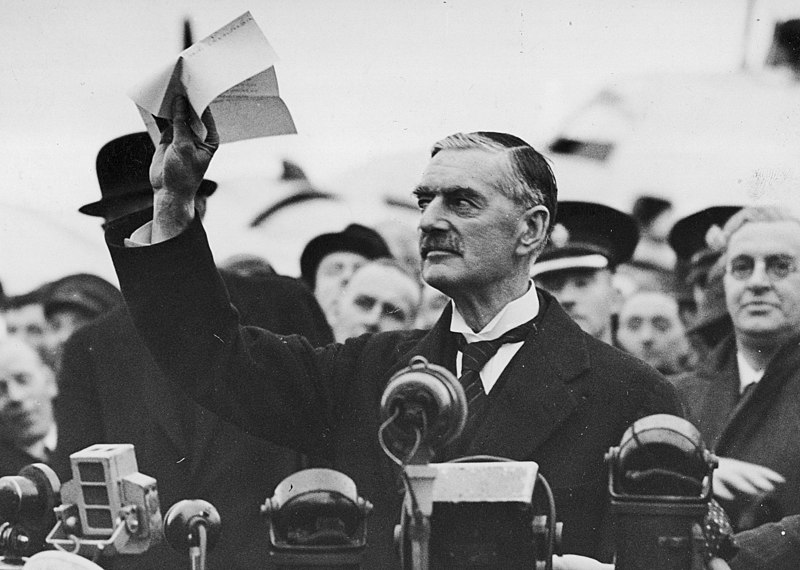
\includegraphics[scale=0.5]{TITLE_IMG}[H]

% %Details
% Jonathan Bittner\\
% IBDP SL Biology\\\\
% Gymnasium Bäumlihof\\
% S. A. Glardon Hansen\\
% 17th February 2023
% \date{}
% \maketitle

% \title {Effects of different energy drinks and their concentration in agarose on \emph{Lepidium sativum} \\[1ex] \large \emph{Red Bull} and \emph{Coop Prix Garantie} energy drinks}
% \maketitle

% \author
% \date{}

% \begin{center}

% \vspace{1cm}

% 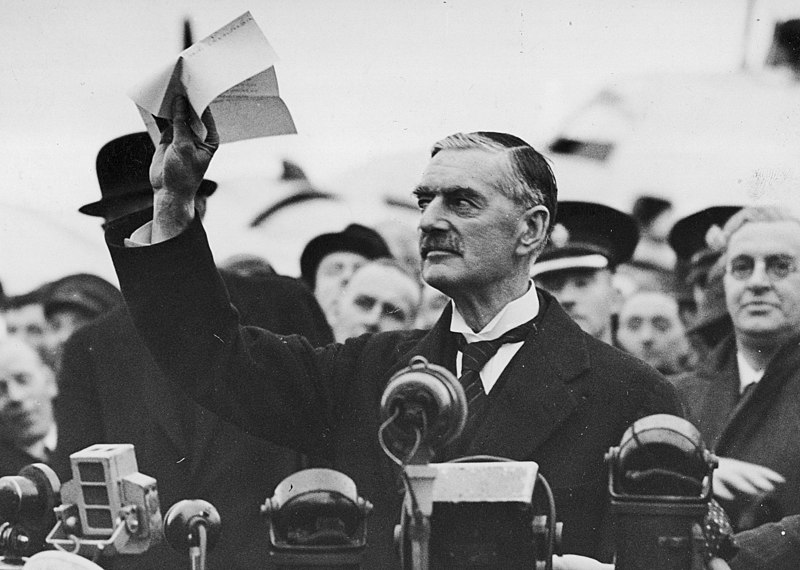
\includegraphics[scale=0.5]{TITLE_IMG}

% \vspace{1cm}


% Jonathan Bittner\\
% IBDP SL Biology\\
% Gymnasium Bäumlihof\\
% S. A. Glardon Hansen\\

% \vspace{1cm}

% \end{center}

% \end{titlepage}

\begin{titlepage}
	\begin{center}
		\vspace*{1cm}
 
		What was Neville Chamberlain's motivation for pursuing the appeasement policy during the Sudetencrisis resulting in the Munich Conference in 1938?
 
		\vspace{0.5cm}
		Neville Chamberlain, the appeasement policy, and the Munich Agreement
			 
		\vspace{1.5cm}
 
		\textbf{Jonathan Bittner}
 
		\vfill
			 
		Internal Assessment
			 
		\vspace{0.8cm}
	  
		% 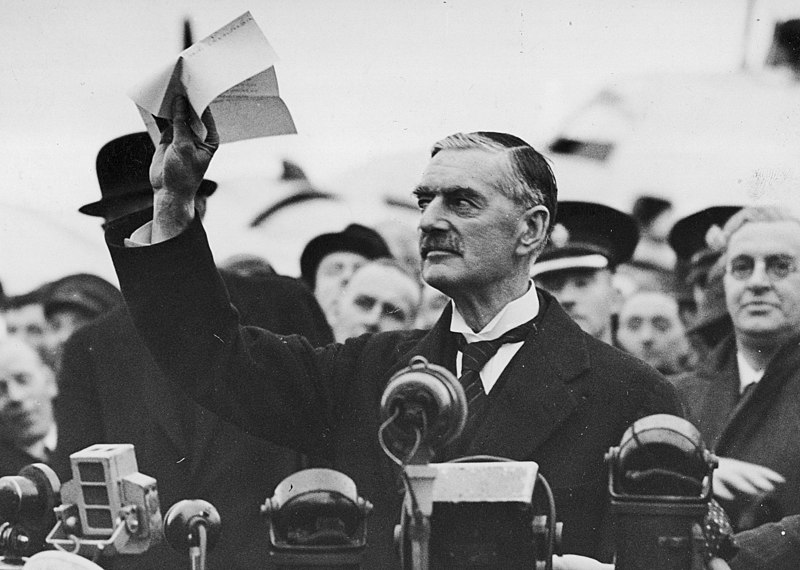
\includegraphics[width=0.6\textwidth]{TITLE_IMG.png}
			 
		IBDP SL History\\
		Gymnasium Bäumlihof\\
		Switzerland\\
		17th February 2023\\
		1453 Words (8. January 23)
			 
	\end{center}
 \end{titlepage}

\tableofcontents
\newpage

\section{Identification and evaluation of sources (497 Words)} % 5 Words

% 41 Words

\emph{Introductory text, w/ research question, state what type of source sources A and B are}\\\\
This investigation will analyze the pursuit of the appeasement policy by Neville Chamberlain in September and October 1938. Following research question will be explored: \emph{What was Neville Chamberlain's motivation for pursuing the appeasement policy during the Sudetencrisis resulting in the Munich Conference in 1938?}. The sources to be evaluated are both primary sources, with N. Chamberlain being the originator.

\subsection{The Neville Chamberlain Diary Letters} % 5 Words

% 204 Words

The first source that will be evaluated is the collection of the diary letters of Neville Chamberlain, written in late 1938. They are addressed to his sisters Hilda and Ida Chamberlain. The letters are valuable because they share insight into Neville Chamberlain's thoughts, better than letters to members of parliament would. The letters have mostly been written in 10 Downing Street, London, and in Chequers, Buckinghamshire. N. Chamberlain wrote the letters to keep in touch, perhaps sometimes persuade and share his thoughts with his sisters. The letters further gain in value, as he comments not only on personal but also on political matters: he shares his 'Plan Z', possible criticism of the British government should war break out, and his hope for resolution of the conflict. A lightly limiting factor of this source are that the letters have been edited by Robert C. Self and published posthumously. This should not have a profound impact on the value, as R. C. Self has worked closely with other historians and also James Lloyd, Neville Chamberlain's grandson \cite{chamberlain_neville_2000}. A further limit is the nature of the source: It is a letter, which can be restricting with what detail N. Chamberlain could have expressed his thoughts and feelings.
%Since these letters have been written by N. Chamberlain, they are biased and show the world from his perspective, something that a historian studying perhaps more than N. Chamberlain's motivations has to accommodate for.

\subsection{Common Sitting, European Situation: Prime Ministers Statement} % 7 Words

%252 Words

% nature\\
The second source to be analyzed is a transcript of Neville Chamberlain's speech to the Members of the House of Commons on September 28th, 1938.
% relevance\\
The transscript is relevant to this investigation because Neville Chamberlain presented his public view on the Sudetencrisis as a Prime Minister, not his personal view.
% origin\\
The speech was held one day before the European powers got together for the Munich Conference, further adding to its value: N. Chamberlain did not present the events in Europe and his views in retrospect -- after the Munich Conference --, which could have changed his views on the situation.
% purpose\\
N. Chamberlain's speech was made to inform the Members of the House of Commons, not necessarily to convince the Members of his actions, because he summarizes the recent events and only draws little attention on his own actions. He also briefly mentions his next move, being his flight to Munich and the get together with other European leaders.
% content\\
There are several limitation concerning this source.
Firstly, the source is a transcript; it leaves room for interpretation in N. Chamberlain's speech. Secondly, it is also possible that the contents of the transcript deviate from the original speech. Thirdly, it could also have been altered on purpose, changing N. Chamberlain's message -- although this seems rather unlikely, as the transcript has been published by the OK Parliament. Lastly, N. Chamberlain's thoughts have been filtered to fit into this speech. To counterbalance this, Source A should reflect his personal thoughts better than Source B does.
\cite{prime_minister_statement_common_sittings_european_situation}

\section{Investigation (943 Words)} % 1 Word
% \subsection{Thesis Statement}

% 77/200 Words

There are numerous possible reasons why N. Chamberlain was motivated to pursue his policy of appeasement. The most notable are Britains military disadvantage, his personal beliefs in finding a peaceful solution and his desire to protect and respect British public opinion. N. Chamberlain's beliefs in peace and the public's opinion are noteworthy, but the military disadvantage of Britain has the most weight in finding the true motivation of Great Britains Prime Minister to pursue the appeasement policy.

\subsection{Military} % 1 Word

% 296/300 Words

Since the beginning of the 1930's Germany had planned to rise to a position of great power in Europe. While they accelerated their rearmament, they also had a détente policy with other European nations. This was to avoid a war of sanctions. By the end of 1937, France and Great Britain had begun to speed up their arming, with the possibility to catch up to the Germans. By mid 1938, the Germans had planned their attack on Czechoslovakia for over 6 months \cite{muenchen_ende_altes_europa}.\\
Germany had developed concrete plans for an attack on Czechoslovakia and Britain was not in a position of power.\\
With no power to carry out your threats, one should never menace, was the conclusion that N. Chamberlain drew from a book on the foreign policy of Canning \cite{chamberlain_neville_2000}. This presents another reason for why N. Chamberlain pursuied the appeasement policy: Great Britain should not menace Germany, as they would not be in a position in which they could carry out their threats.\\
Furthermore, N. Chamberlain stated that Great Britain was in no position in which "[their] military advisors would feel happy in undertaking hostilities if we were not forced to do so" \cite{chamberlain_neville_2000}. With no support from government officials, a war against Germany would be impossible. In addition to this, the British Cabinet received a note from Ismay Hastings -- a general in the British Indian Army -- about how it would be favourable to delay a potential war with Germany for about six to twelve months:\\\\
"It follows, therefore, that, from the military point of view, time is in our favour, and that, if war with Germany has to come, it would be better to fight her in say 6-12 months’ time, than to accept the present challenge." \cite{ismay1938}

% \subsection{Letters to His Sisters}
\subsection{Pacifism} % 1 Word

% 279/300 Words

% N. Chamberlain's motivation to prevent war is evident is the letters to his sisters, where he showed his dedication to finding a peaceful solution to the Sudetencrisis. He states in a letter written on September 11th, 1938 that the Daily Mail had declared that the United Kingdom had issued an ultimatum to Germany. N. Chamberlain had to publicly deny this and described this action of the Daily Mail as "most gratuitously mischievous"; this implies that he would never pass such a measure. This expresses a clear stance towards a possible conflict with Germany, and N. Chamberlain's push to find a peaceful solution to the Sudetencrisis. He also stated that .\\
% Furthermore, N. Chamberlain expressed in a letter written eight days later, that he did not care wether the Sudetenland was in the German Reich or not. This again demonstrates his will to find a settlement to which both Czechoslovakia and Germany could agree.\\
% % This shows his desire to find a peaceful solution and his will to prevent the terror of war.
% Nevertheless, N. Chamberlain implied,  in a letter written on October 9th, that he felt a moral obligation to protect weaker nations from Germany, which was taking advantage of them: He wrote in this letter that he "had to fight all the time against the [sic] defection of weaker brethrens".

N. Chamberlain's motivation to prevent war is evident in the letters to his sisters: He showed dedication to find a peaceful solution to the Sudetencrisis. He stated in a letter written on September 11th, 1938 that the Daily Mail had declared that the United Kingdom had issued an ultimatum to Germany. N. Chamberlain called this action "most gratuitously mischievous of all", taking a clear stance not only to the action of the Daily Mail but also against a possible ultimatum.\\
Furthermore, N. Chamberlain expressed in a letter written eight days later, that he did not care wether the Sudetenland was in the German Reich or not. This not only shows his will to find a settlement to which both Czechoslovakia and Germany could agree, but also shows that he did not want to risk a war for the Sudetens.\\
Another demonstration of his pacifist conviction is, that he not only let Lord Runciman, and later Sir Horace Wilson, handle this conflict; N. Chamberlain had planned to surprise Hitler with the offer to meet him when things looked darkest and the crisis seemed to reach its climax. This was without consent of Monsieur Daladier -- the French Prime Minister -- and also a surprise to the Members of the House of Commons \cite{voelkerbund_muenchener_abkommen_hermann_raschhofer}. He tried an unconventional method, in a moment when things looked as if nothing could be done, to prevent war.\\
He stayed with his peaceful solution even when other politicians (Winston Churchill and Tomáš Masaryk) carried out a conspiracy against him \cite{chamberlain_neville_2000}, which he wrote on October 9th, 1938. It stays unclear wether this was out of hopes to increase his popularity among the politicans and the public or wether it is a testament to his belief in finding a conflict-free and sustainable solution for the Sudetencrisis.


% \subsection{Speech to Members of the House of Commons}
\subsection{Britain's Public Opinion} % 3 Words

% 210/300 Words

% In the speech to the Members of the House of Commons, N. Chamberlain advocated for the same political program he described in the letters to his sisters. The actions he had taken and described in his letters were also present in his speech. He takes a clear stance in his letters, whereas in his speech he presents it in a neutral manner. This is especially clear in the following extract of the speech's transcript, where he describes his first meeting with Hitler on September 15th 1938:\\\\
% "On that he said that if I could give him there and then an assurance that the British Government accepted the principle of self-determination he would be quite ready to discuss ways and means of carrying it out" \cite{prime_minister_statement_common_sittings_european_situation}\\\\
% This statement is also found in a letter written four days later, in almost the same wording. In his letter, N. Chamberlain inserts his personal opinion right after this statement. This is a notable difference, as he did not do this in his speech:\\\\
% "My personal opinion was that on principle I didn't care two hoots wether the Sudetens were in the Reich or out of it [but saw difficulties in a plebiscite]" \cite{chamberlain_neville_2000}\\\\
% That the content of his speech to the House of Commons and the letters to his sisters are very similar -- with the difference that he left his personal opinion out of the speech -- suggests, that he meant what he said in his speech. Following this thesis, it can be said that his political appeasement program was out of personal conviction.

N. Chamberlain was also motivated by the desire to protect Britain's interests and respect the public's opinion against war. This is especially clear in his speech to the House of Commons on September 28th, 1938: With the statement that "this country, which does not readily resort to war, would not have followed us if we had tried to lead it into war to prevent a  minority from obtaining autonomy, or even from choosing to pass under some other Government." \cite{prime_minister_statement_common_sittings_european_situation} he explains that charging into war with Germany would have not been supported by the british public. He also stated that Great Britain "does not readily resort to war" \cite{chamberlain_neville_2000}. It has to be said that this is not tied to the public's opinion but more with a country's political orientation, beliefs and strategy, which in Great Britain's case was not pro-war.\\
Polls taken after the Munich Conference showed that 57\% of people were satisfied with the results. This implies that these people preferred peace over war. However, in a different poll, 72\% of people were in still in favor of an increased defense spending after the Munich Conference. Given these results, it can be said that the British public distrusted Germany and Hitler, but nonetheless preferred peace over war.

\subsection{Conclusion}

% 200 Words

Britain's public opinion and his own beliefs in a peaceful solution to the Sudetencrisis are influential factors that have determined N. Chamberlain's motivation for his appeasement policy. The most crucial factor influencing his will to find a peaceful solution is Britains military disadvantage compared to Germany. With not only his closest advisors but also members from within the military advocating against a war, it sent a clear signal to N. Chamberlain to keep pushing for a non-violent resolution of the crisis.

\section{Reflection (0 Words)}


\newpage
\section{Bibliography}
\printbibliography[heading=none]
\end{document}